\documentclass[a4paper]{article}
\usepackage{times}
\usepackage{mathptmx}
\usepackage[boldfont,slantfont]{xeCJK}
\setmainfont{Times New Roman}
\setsansfont{Times New Roman}
\setCJKmainfont{宋体}
\setCJKsansfont{黑体}
\setCJKmonofont{仿宋}
\setCJKfamilyfont{hei}{黑体}
\setCJKfamilyfont{kai}{楷体}
\newcommand{\hei}{\CJKfamily{hei}}
\newcommand{\kai}{\CJKfamily{kai}}
\usepackage{amsmath,amssymb,amsthm}
\usepackage{geometry}
\geometry{left=2.5cm,right=2.5cm,top=2.5cm,bottom=2.5cm}
\usepackage{fancyhdr}
\usepackage{lastpage}
\usepackage{array}
\usepackage{pgf,tikz}
\usetikzlibrary{calc,intersections}
\usetikzlibrary{arrows,snakes,backgrounds}
\usetikzlibrary{shapes.geometric}
\pgfmathdeclarefunction{fix}{1}{\global \pgfmathunitsdeclaredfalse}
\newcommand{\tabincell}[2]{\begin{tabular}{@{}#1@{}}#2\end{tabular}} 
\def\leq{\leqslant}
\def\geq{\geqslant}
\def\byh{\!\!“}
\def\eyh{”\!\!}
\begin{document}
    \renewcommand{\baselinestretch}{1.25}\normalsize
    \setlength{\parindent}{2em}
    \setlength{\abovedisplayskip}{1pt}
    \setlength{\belowdisplayskip}{1pt}
    \pagestyle{fancy}
    \fancyhf{}
    \fancyhead[l]{NOIP提高班——数学专项练习}
    \fancyhead[r]{2018年2月22日}
    \fancyfoot[c]{第\thepage 页\qquad 共\pageref{LastPage} 页}
    \renewcommand{\headrulewidth}{0.1mm}

    \begin{center}
        {\LARGE \hei NOIP提高班——数学专项练习}

        {\kai (请选手务必仔细阅读本页内容)}
    \end{center}

    {\bf 一、题目概况}

    \begin{center}
        \begin{tabular}{|*{4}{p{3.5cm}<{\centering}|}}
            \hline
            中文题目名称 & 哈希函数 & 向量 & 仪仗队 \\\hline
            英文题目与子目录名 & hash & vector & honourguard \\\hline
            可执行文件名 & hash & vector & honourguard \\\hline
            输入文件名 & hash.in & vector.in & honourguard.in \\\hline
            输出文件名 & hash.out & vector.out & honourguard.out \\\hline
            每个测试点时限 & 1秒 & 1秒 & 2秒 \\\hline
            测试点数目 & 10 & 10 & 10 \\\hline
            每个测试点分值 & 10 & 10 & 10 \\\hline
            附加样例文件 & 有 & 有 & 有 \\\hline
            结果比较方式 & \multicolumn{3}{c|}{全文比较(过滤行末空格及文末回车)} \\\hline
            题目类型 & 传统 & 传统 & 传统 \\\hline
            运行内存上限 & 256M & 256M & 1G \\\hline
        \end{tabular}
    \end{center}

    {\bf 二、提交源程序文件名}

    \begin{center}
        \begin{tabular}{|*{4}{p{3.5cm}<{\centering}|}}
            \hline
            对于 \makebox[28pt][l]{C++}语言 & hash.cpp & vector.cpp & honourguard.cpp \\\hline
            对于 \makebox[28pt][l]{C}语言 & hash.c & vector.c & honourguard.c \\\hline
            对于 \makebox[28pt][l]{Pascal}语言 & hash.pas & vector.pas & honourguard.pas \\\hline
        \end{tabular}
    \end{center}

    {\bf 三、编译命令(不包含任何优化开关)}

    \begin{center}
        \begin{tabular}{|*{4}{p{3.5cm}<{\centering}|}}
            \hline
            对于 \makebox[28pt][l]{C++}语言 & g++ -o hash hash.cpp -lm & g++ -o vector vector.cpp -lm & g++ -o honourguard honourguard.cpp -lm \\\hline
            对于 \makebox[28pt][l]{C}语言 & gcc -o hash hash.c -lm & gcc -o vector vector.c -lm & gcc -o honourguard honourguard.c -lm \\\hline
            对于 \makebox[28pt][l]{Pascal}语言 & fpc hash.pas & fpc vector.pas & fpc honourguard.pas \\\hline
        \end{tabular}
    \end{center}

    {\bf 注意事项:\!\!}

    1. 文件名(程序名和输入输出文件名)必须使用英文小写;\!\!

    2. C/C++中函数main()的返回值类型必须是int,\!\!程序正常结束时的返回值必须是0;\!\!

    3. 只提供Linux格式附加样例文件.

    \newpage

    \begin{center}
        \Large \hei 1. 哈希函数

        {\ttfamily (hash.cpp/c/pas)}
    \end{center}

    【问题描述】

    明明觉得hash是个好算法,\!\!代码短、效率高. 某天,\!\!他碰到了一个求正方形个数的问题,\!\!于是很淡定地枚举对角线,\!\!然后用hash判存在,\!\!妥妥的搞定,\!\!但是提交后却wa了几个点. 仔细观察其hash函数为:\!\!$h=xy+x+y$. 为了让明明知道这个函数存在什么问题,\!\!对于给出一个$h$值,\!\!请你来告诉他有多少对$(x,y)$满足上述式子$(\max\{x,y\}\leq h$;\!\!$h,x,y$都为非负整数$)$?

    【输入格式】

    输入文件名为{\ttfamily hash.in}.

    输入文件第一行包含一个正整数$T$,\!\!表示数据组数.

    接下来$T$行每行包含一个整数$h$,\!\!意义详见题目描述.

    【输出格式】

    输出文件名为{\ttfamily hash.out}.

    输出文件包含$T$行,\!\!每行一个整数,\!\!分别表示有多少组$(x,y)$满足要其对应的$h$值.

    【输入输出样例1】

    \begin{tabular}{|*{2}{p{5cm}|}}
        \hline
        {\ttfamily hash.in} & {\ttfamily hash.out} \\\hline
        \tabincell{l}{3\\1\\3\\4} & \tabincell{l}{2\\3\\2\\~~} \\\hline
    \end{tabular}

    【输入输出样例1说明】

    第一组:\!\!$(1,0),(0,1)$.

    第二组:\!\!$(0,3),(1,1),(3,0)$.

    第三组:\!\!$(4,0),(0,4)$.

    【输入输出样例2】

    见选手目录下的{\ttfamily hash/hash2.in}和{\ttfamily hash/hash2.ans}.

    【数据规模与约定】

    对于30\%的数据,\!\!$h\leq 2,000$,\!\!$T\leq 1,000$.

    对于70\%的数据,\!\!$h\leq 10,000$,\!\!$T\leq 10,000$.

    对于100\%的数据,\!\!$h\leq {10}^8$,\!\!$T\leq 10,000$.

    \newpage

    \begin{center}
        \Large \hei 2. 向量

        {\ttfamily (vector.cpp/c/pas)}
    \end{center}

    【问题描述】

    给你一对数$a,b$,\!\!你可以任意使用$(a,b),(a,-b),(-a,b),(-a,-b),(b,a),(b,-a),(-b,a),(-b,-a)$这些向量,\!\!问你能不能拼出另一个向量$(x,y)$.

    说明:\!\!这里的拼就是使得你选出的向量之和为$(x,y)$.

    【输入格式】

    输入文件名为{\ttfamily vector.in}.

    输入文件第一行包含一个正整数$T$,\!\!为数据的组数.

    接下来$T$行每行包含四个整数$a,b,x,y$.

    【输出格式】

    输出文件名为{\ttfamily vector.out}.

    输出文件包含$T$行,\!\!每行为\byh Y\eyh 或\byh N\eyh ,\!\!分别表示可以拼出来、不能拼出来.

    【输入输出样例1】

    \begin{tabular}{|*{2}{p{5cm}|}}
        \hline
        {\ttfamily vector.in} & {\ttfamily vector.out} \\\hline
        \tabincell{l}{3\\2 1 3 3\\1 1 0 1\\1 0 -2 3} & \tabincell{l}{Y\\N\\Y\\~~} \\\hline
    \end{tabular}

    【输入输出样例1说明】

    第一组:\!\!$(2,1)+(1,2)=(3,3)$.

    第二组不能拼成.

    第三组:\!\!$(-1,0)+(-1,0)+(0,1)+(0,1)+(0,1)=(-2,3)$.

    【输入输出样例2】

    见选手目录下的{\ttfamily vector/vector2.in}和{\ttfamily vector/vector2.ans}.

    【数据规模与约定】

    对于100\%的数据,\!\!$T\leq 500,000$,\!\!$-2\times {10}^9\leq a,b,x,y\leq 2\times{10}^9$.

    \newpage

    \begin{center}
        \Large \hei 3. 仪仗队

        {\ttfamily (honourguard.cpp/c/pas)}
    \end{center}

    【问题描述】

    作为体育委员,\!\!C君负责这次运动会仪仗队的训练. 仪仗队是由学生组成的$N\times N$的方阵,\!\!为了保证队伍在行进中整齐划一,\!\!C君会跟在仪仗队的左后方,\!\!根据其视线所及的学生人数来判断队伍是否整齐(如下图). 现在,\!\!C君希望你告诉他队伍整齐时能看到的学生人数.

    \begin{center}
        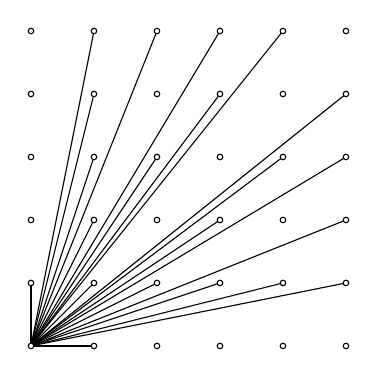
\begin{tikzpicture}[scale=0.8]
            \draw (0,0)--(1,0);
            \draw (0,0)--(0,1);
            \draw (0,0)--(1,1);
            \draw (0,0)--(2,1);
            \draw (0,0)--(3,1);
            \draw (0,0)--(4,1);
            \draw (0,0)--(5,1);
            \draw (0,0)--(1,2);
            \draw (0,0)--(3,2);
            \draw (0,0)--(5,2);
            \draw (0,0)--(1,3);
            \draw (0,0)--(2,3);
            \draw (0,0)--(4,3);
            \draw (0,0)--(5,3);
            \draw (0,0)--(1,4);
            \draw (0,0)--(3,4);
            \draw (0,0)--(5,4);
            \draw (0,0)--(1,5);
            \draw (0,0)--(2,5);
            \draw (0,0)--(3,5);
            \draw (0,0)--(4,5);
            \foreach \x in {0,1,...,5}
                \foreach \y in {0,1,...,5}
                    \draw [fill=white] (\x,\y) circle (1/0.8pt);
        \end{tikzpicture}
    \end{center}

    【输入格式】

    输入文件名为{\ttfamily honourguard.in}.

    输入数据仅一行,\!\!包含一个正整数$N$,\!\!表示方阵的边长.

    【输出格式】

    输出文件名为{\ttfamily honourguard.out}.

    输出文件仅一行,\!\!包含一个正整数$M$,\!\!为C君应看到的学生人数.

    【输入输出样例1】

    \begin{tabular}{|*{2}{p{5cm}|}}
        \hline
        {\ttfamily honourguard.in} & {\ttfamily honourguard.out} \\\hline
        4 & 9 \\\hline
    \end{tabular}

    【输入输出样例1说明】

    \begin{center}
        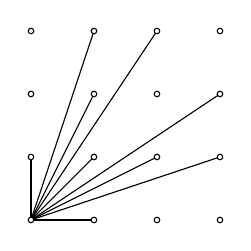
\begin{tikzpicture}[scale=0.8]
            \draw (0,0)--(1,0);
            \draw (0,0)--(0,1);
            \draw (0,0)--(1,1);
            \draw (0,0)--(2,1);
            \draw (0,0)--(3,1);
            \draw (0,0)--(1,2);
            \draw (0,0)--(3,2);
            \draw (0,0)--(1,3);
            \draw (0,0)--(2,3);
            \foreach \x in {0,1,2,3}
                \foreach \y in {0,1,2,3}
                    \draw [fill=white] (\x,\y) circle (1/0.8pt);
        \end{tikzpicture}
    \end{center}

    【输入输出样例2】

    见选手目录下的{\ttfamily honourguard/honourguard2.in}和{\ttfamily honourguard/honourguard2.ans}.

    【数据规模与约定】

    对于30\%的数据,\!\!$1\leq N\leq 1,000$.

    对于70\%的数据,\!\!$1\leq N\leq 40,000$.

    对于100\%的数据,\!\!$1\leq N\leq 40,000,000$.
\end{document}